\documentclass[a4paper,english,12pt]{article}
\usepackage{%
	amsmath,%
	amsfonts,%
	amssymb,%
	amsthm,%
	hyperref,%
	url,%
	latexsym,%
	epsfig,%
	graphicx,%
	psfrag,%
	subfigure,%	
	color,%
	tikz,%
	pgf,%
	pgfplots,%
	pgfplotstable,%
	pgfpages,%
	proofs%
}

\usepgflibrary{shapes}
\usetikzlibrary{%
  arrows,%
	backgrounds,%
	chains,%
	decorations.pathmorphing,% /pgf/decoration/random steps | erste Graphik
	decorations.text,%
	matrix,%
  positioning,% wg. " of "
  fit,%
	patterns,%
  petri,%
	plotmarks,%
  scopes,%
	shadows,%
  shapes.misc,% wg. rounded rectangle
  shapes.arrows,%
	shapes.callouts,%
  shapes%
}

\theoremstyle{plain}
\newtheorem{thm}{Theorem}[section]
\newtheorem{lem}[thm]{Lemma}
\newtheorem{prop}[thm]{Proposition}
\newtheorem{cor}[thm]{Corollary}

\theoremstyle{definition}
\newtheorem{defn}[thm]{Definition}
\newtheorem{conj}[thm]{Conjecture}
\newtheorem{exmp}[thm]{Example}
\newtheorem{assum}[thm]{Assumptions}

%\theoremstyle{remark}
\newtheorem{rem}{Remark}
\newtheorem{note}{Note}

\makeatletter
\def\th@plain{%
  \thm@notefont{}% same as heading font
  \itshape % body font
}
\def\th@definition{%
  \thm@notefont{}% same as heading font
  \normalfont % body font
}
\makeatother
\date{}
%\usepackage[T1]{fontenc}
%\PassOptionsToPackage{normalem}{ulem}
%\makeatletter

\begin{document}

\title{Lecture 5: Functions : Images, Compositions, Inverses}
\author{}
\maketitle

\section{Functions}
We have all seen some form of functions in high school. For example, we have seen polynomial, exponential, logarithmic, trigonometric functions in calculus. These functions map real numbers to real numbers. We have also seen functions that map functions to functions, such a derivatives. Functions are of interest in many branches of mathematics, including enumerative combinatorics, topology, and group theory among others. An abstract understanding of function would be, an output $f(x)$ for each input $x$. We formalize this notion below.
\begin{defn} [Function]
 Let $A$ and $B$ be sets. A \textbf{function} (also called a \textbf{map}) from $A$ to $B$ denoted $f: A \to B$ is a subset $F \subseteq A \times B$ such that for each $a \in A$, there is a unique pair of the form $(a,b)$ in $F$. The set $A$ is called the domain of $f$ and the set $B$ is called the co-domain of $f$.
\end{defn}

\begin{rem} To show the equality of functions, we need to show that the domain, co-domain, and subset of the product of domain and co-domain satisfying the given condition imposed by function $f$, all three must agree.
\end{rem}

\begin{defn}
Let $A$ and $B$ be sets, and let $S \subseteq A$ be a subset. 
\begin{enumerate}
 \item  A \textbf{constant map} $f: A \to B$ is any function of the form $f(x) = b$ for all $x \in A$, where $b \in B$ is some fixed element.
 
 \item  The \textbf{identity map} on $A$ is the function $1_{A}: A \to A$ defined by $1_{A}(x) = x$ for all $x \in A$.

 \item  The \textbf{inclusion map} from $S \to A$ is the function $j: S \to A$ defined by $j(x) = x$ for all $x \in A$.

 \item If $f: A \to B$ is a map, the \textbf{restriction} of $f \to S$, denoted by $f |_{S}$ is the map $f|_{S}: S \to B$, defined by $f|_{S}(x)= x$ for all  $x \in S$.

 \item  If $g: A \to B$ is a map, an \textbf{extension} of $g$ to $A$ is any map $G: A \to B$ such that $G|_{s} = g$.

 \item   The \textbf{projection maps} from $A \times B$ are the functions, $\pi_{1}: A \times B \to A$ and $\pi_{2}: A \times B \to B$ defined by $\pi_{1}(a, b) = a$ and $\pi_{2}(a, b) = b$ for all $(a,b) \in A \times B$. Projection maps $\pi_{i}: A_{1} \times A_{2} \times \dots \times A_{p} \to A_{i}$ for  any finite collection of sets $A_{1}, A_{2} \dots A_{p}$ are defined similarly.
\end{enumerate}
\end{defn}

\section{Image and Inverse Image}

\begin{defn} [Image and inverse image]
 Let $f: A \to B$ be a function.
 \begin{enumerate}
  \item For each $P\subseteq A$, the \textbf{image} of $P$ under $f$ is defined as
\begin{equation*}
f(P)  =\{b\in B: b=f(p) \textnormal{ for some } p\in P\} =\{f(p):p\in P\}.
\end{equation*}
%The \textbf{range} (image) of $f$ is the set $f(A)$.
  \item For each $Q\subseteq B$, the \textbf{inverse image} (or \textbf{preimage}) of $Q$ under $f$ is defined as
\begin{equation*}
f^{-1}(Q)  =\{a\in A: f(a)=q \textnormal{ for some } q\in Q\} =\{a\in A:f(a)\in Q\}
\end{equation*}
 \end{enumerate}
\end{defn}
\begin{figure}[hhh]
\centering
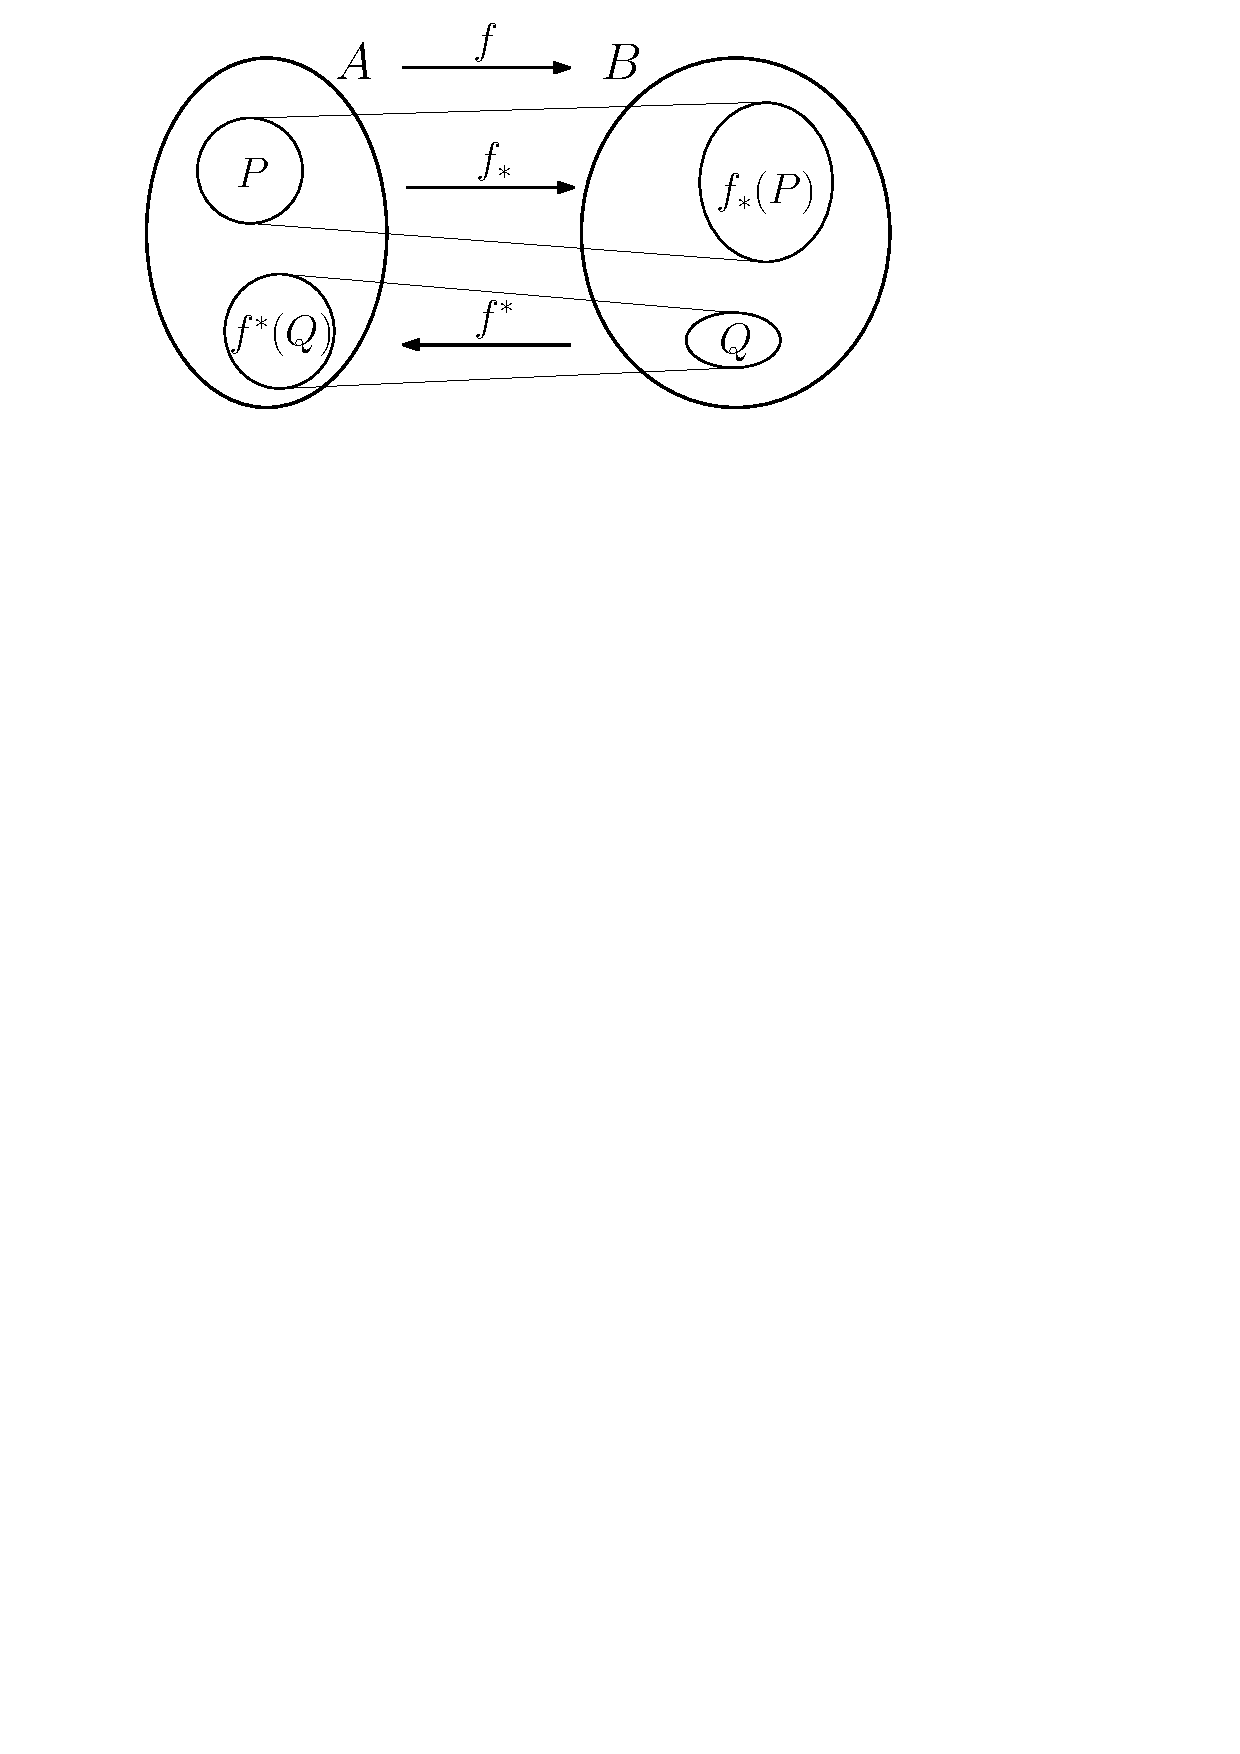
\includegraphics[scale=0.6]{Figures/l5f1_img-invimg.pdf}
\caption{Image and inverse image under a function $f$.}
\end{figure}

\begin{rem} Let $f: A \to B$ be a function.
\begin{enumerate}[i)]
\item For every $\emptyset \neq P\subseteq A$, $\emptyset \neq f(P)\subseteq B$ and $|P|\geqslant |f(P)|$. 
\item The \textbf{range} (or \textbf{image}) of $f$ is the set $f(A)$. The range need not be equal to the co-domain.
\item For every $Q\subseteq B$, $f^{-1}(Q)\subseteq A$, possibly be empty, and $|Q|\leqslant |f^{-1}(Q)|$. 
\item Given a function $f:A \to B$, the process of taking image of subsets of $A$ can be thought of as operation of a function $f_{\ast}:\mathcal{P}(A)\to \mathcal{P}(B)$ on subsets of $A$ and induced by $f$.
\item Given a function $f: A \to B$, the process of taking inverse image of subsets of $B$ can be thought of as operation of a new function $f^{\ast}:\mathcal{P}(B) \to \mathcal{P}(A)$ on subsets of $B$ and induced by $f$.
\item Abuse of notation: 
\begin{enumerate}[a)]
\item Notice that $f$ maps elements in $A$ to elements in $B$, and $f_{\ast}$ maps subsets of $A$ to subsets of $B$. Following common convetions, we will use $f$ for $f_{/ast}$. 
%Even though $f$ maps elements of $A$ to elements of $B$ and not subsets of $A$ (say $P$) to subsets of $B$ (say $Q$), often $f$ is replaced with $f$ for convenience, \textit{i.e.}, $f(P)$ is substituted for $f(P)$.
\item Similarly, $f^{\ast}$ is replaced with $f^{-1}$ for inverse image. 
\item Later, we will look at the \textbf{inverse} of a function $f:A \to B$ (if it exists) and denote it by $f^{-1} : B \to A$. If the inverse function of $f$ does not exist, then $f^{-1}(Q)$ is used to refer to the inverse image $f^{-1}(Q)$ of $Q$ under $f$. If the inverse of $f$ exists, then it takes elements and not subsets of $B$ as the argument, and $f^{-1}(Q)=f^{\ast}(Q)=f^{-1}_*(Q)$. That is, $f^{-1}(Q)$ can be used to refer to both the inverse image $f^{\ast}(Q)$ of $Q$ under $f$ and the image $f^{-1}_*(Q)$ of $Q$ under $f^{-1}$.
\end{enumerate}
\end{enumerate}
\end{rem}

\begin{exmp}
Consider the function $f:\mathbb{R}\rightarrow \mathbb{R}$ plotted in Figure~\ref{func_ex}.\begin{enumerate}[i)]
\item The range of $f$, $f(\mathbb{R})=[-3,\infty)\subset \mathbb{R}$.
\item For $P_1=[1.5,1.9]$ and $P_2=[-4.5,-3.3]$, $f(P_1)=[1.7,2.5]$ and $f(P_2)=[-3,-1]$.
\begin{figure}[h]
\centering
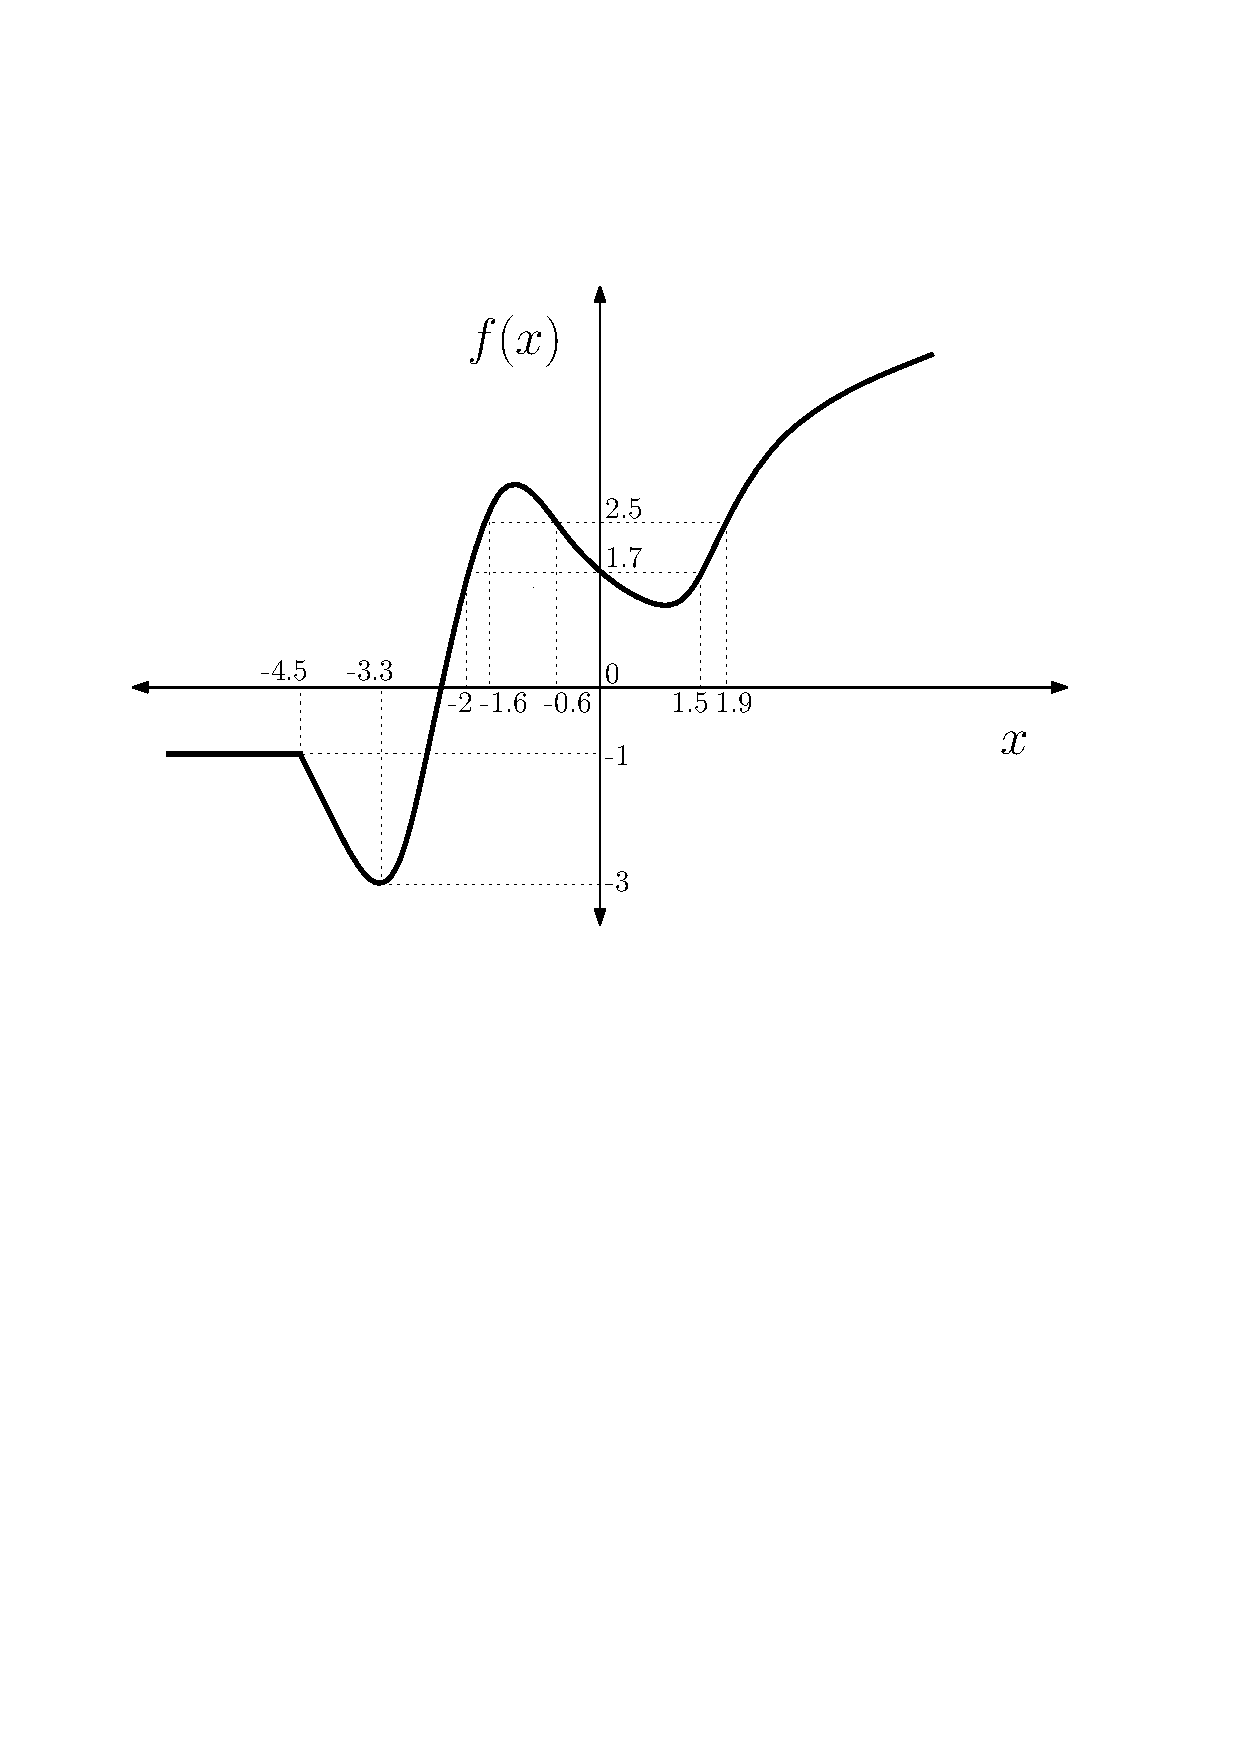
\includegraphics[scale=0.6]{Figures/l5f2_graph.pdf}
\caption{Example function.}
\label{func_ex}
\end{figure}
\item For $Q_1=[1.7,2.5]$ and $Q_2=[-4,-3.2]$, $f^{-1}(Q_1)= [-2,-1.6] \cup [-0.6,0] \cup [1.7,2.5]$ and $f^{-1}(Q_2)=\emptyset$.
\item From (i) and (ii), we have that $f^{-1}(f(P_1))\neq P_1$, $f^{-1}(f(P_2))=P_2$, $f(f^{-1}(Q_1))=Q_1$ and $f(f^{-1}(Q_2))=Q_2$ (cf. Theorem~\ref{img-preimg_props}).
\end{enumerate}
\end{exmp}

We state the following theorem with proof left as an exercise to the reader. Most of the proofs require showing set equality using set inclusions.
\begin{thm} Let $A$ and $B$ be sets, let $C,D\subseteq A$ and $S,T\subseteq B$ be subsets of $A$ and $B$ respectively, and let $f:A \to B$ be a function. Let $I,J\neq\emptyset$, let $\{U_i:i \in I\}$ and $\{V_j:j \in J\}$ be indexed families of sets, where $U_i \subseteq A$, for all $i \in I$ and $V_j \subseteq B$, for all $j \in J$.
\begin{multicols}{2}
\begin{enumerate}[i)]
\item $f(\emptyset)=\emptyset$ and $f^{-1}(\emptyset)=\emptyset$.
\item $f^{-1}(B)=A$.
\item $f(C)\subseteq S$ iff $C\subseteq f^{-1}(S)$.
\item If $C\subseteq D$, then $f(C)\subseteq f(D)$.
\item If $S\subseteq T$, then $f^{-1}(S)\subseteq f^{-1}(T)$.
\item $f(\bigcup_{i\in I}U_i)=\bigcup_{i\in I}f(U_i)$.
\item $f(\bigcap_{i\in I}U_i)\subseteq \bigcap_{i\in I}f(U_i)$.
\item $f^{-1}(\bigcup_{j\in J}V_j)=\bigcup_{j\in J}f^{-1}(V_j)$.
\item $f^{-1}(\bigcap_{j\in J}V_j)=\bigcap_{j\in J}f^{-1}(V_j)$.
\end{enumerate} 
\end{multicols}
\label{img-preimg_props}
\end{thm}
%\begin{proof}
%%%(\textit{Hint: Let $X$ and $Y$ be sets. To show $X=Y$, show that $X\subseteq Y$ and $Y\subseteq X$.})
%%\begin{enumerate}[i)]
%%\item Follows trivially from definition of empty sets.
%%\item By definition, $f^{-1}(B) \subseteq A$. Since $f$ maps each element in domain $A$ to some element in $B$, we have $A \subseteq f^{-1}(B)$ .
%%\end{enumerate}
%\end{proof}

\section{Composition of Function}
We are interested in combining functions to create more interesting functions. Addition and multiplication of functions is not defined on arbitrary sets. However, as we will see in this section, combination is a natural way to define new functions on arbitrary sets.
\begin{defn}[Composition of Functions] Let $A$, $B$ and $C$ be sets, and let $f:A\to B$ and $g:B \to C$ be functions. The \textbf{composition} of $f$ and $g$ is the function $g\circ f:A \to C$ defined as
\begin{equation*}
(g \circ f) (x)  =g(f(x)) \text{ for all } x\in A.
\end{equation*}
\end{defn}

Function compositions can be visualized by \textbf{commutative diagrams}. Figure~\ref{Fig:CommDiag} has the commutative diagram for $g\circ f$.
\begin{figure}[hhhh]
\centering
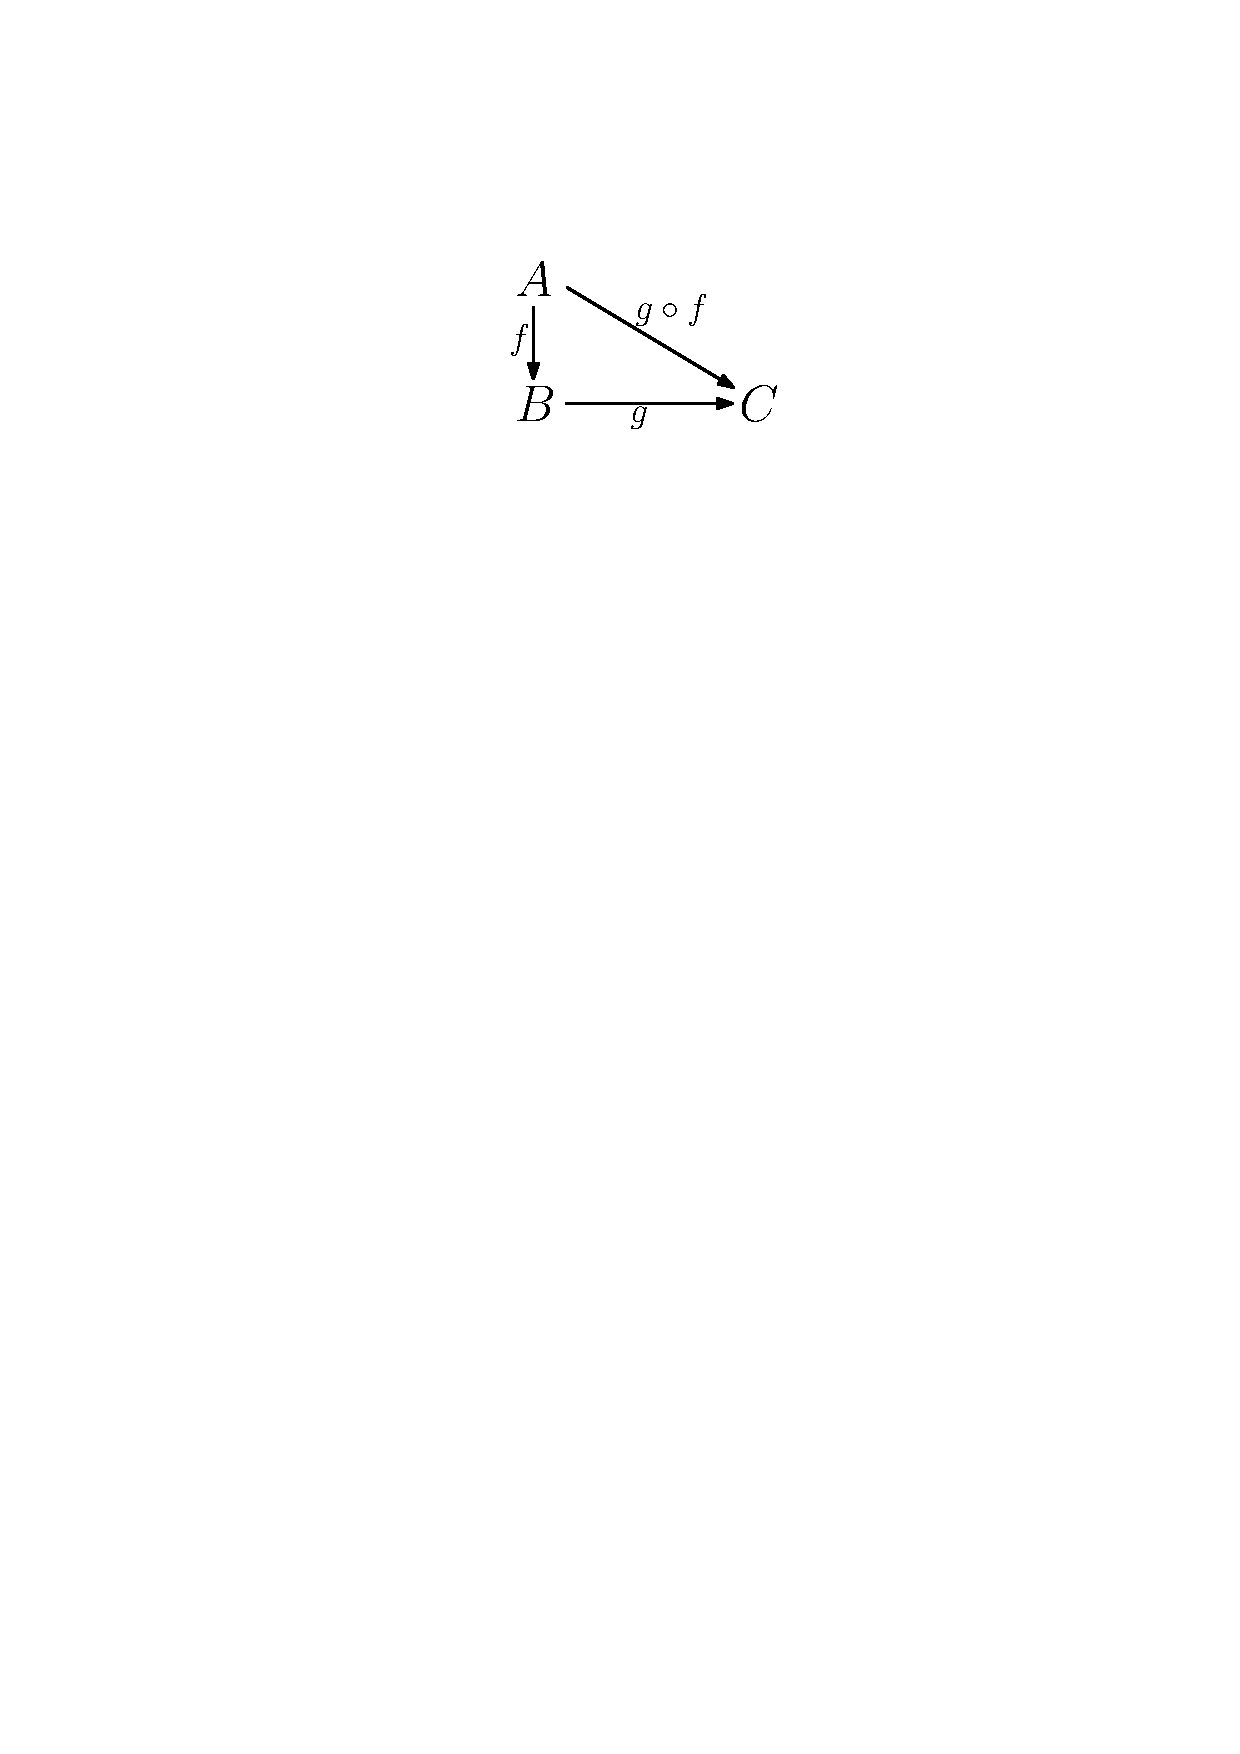
\includegraphics[scale=0.8]{Figures/l5f3_commdiag.pdf}
\caption{Commutative diagram for $g \circ f$.}
\label{Fig:CommDiag}
\end{figure}

\begin{rem} Let $f : A \to B$ and $g: B \to C$ be functions.
\begin{enumerate}[i)]
\item Composition of three or more functions can be defined similarly.
\item Though read/written left to write, while obtaining value of $(g\circ f)(a),a\in A$, $f(a)$ is computed first followed by $g(f(a))$.
%\item 
\item %If the co-domain of the $f$ is subset of the domain of $g$, then the composition $g \circ f$ is defined. %(
The composition $g \circ f$ is defined iff the range of $f$ is a subset of the domain of $g$.
\item If $A=C$, then $f \circ g$ is also defined but need not necessarily be equal to $g\circ f$ or $1_A$.
\item The range of $g \circ f$ is a subset of range of $g$. That is, $(g\circ f)(A) \subseteq g(B)$.
\end{enumerate}
\end{rem}

\begin{exmp}
Let $f:\mathbb{R}\rightarrow \mathbb{R}$ be defined by $f(x)=x^3$ , $g:[0,\infty)\rightarrow \mathbb{R}$ be defined by $g(x)=\sqrt{x}$ and $h:\mathbb{R}\rightarrow \mathbb{R}$ be defined by $h(x)=2x$. Then 
\begin{enumerate}[i)]
\item $f\circ f:\mathbb{R}\rightarrow \mathbb{R}$ and $(f\circ f)(x)=(x^3)^3$.
\item $(f\circ g):[0,\infty)\rightarrow \mathbb{R}$ and $(f\circ g)(x)=\sqrt{x^3}$.
\item $(f\circ h):\mathbb{R}\rightarrow \mathbb{R}$ and $(f\circ h)(x)=(2x)^3$.
\item $(h\circ f):\mathbb{R}\rightarrow \mathbb{R}$ and $(h\circ f)(x)=2x^3$. (Note that $(h\circ f)\neq (f\circ h)$)
\item $(h\circ g):[0,\infty)\rightarrow \mathbb{R}$ and $(h\circ g)(x)=2\sqrt{x}$.
\item $f\circ h\circ g:[0,\infty)\rightarrow \mathbb{R}$ and $(f\circ h\circ g)(x)=(2\sqrt{x})^3$.
\item $f\circ f\circ h:\mathbb{R}\rightarrow \mathbb{R}$ and $(f\circ f\circ h)(x)=((2x)^3)^3$.
\item $(g\circ g),\,(g\circ f),\,(g\circ h),\,(f\circ g\circ h),\,(g\circ h\circ f),\,(g\circ f\circ h),\,(h\circ g\circ f)$ are not defined.
\end{enumerate}
Similarly, many more functions can be obtained.
\label{ex_comp}
\end{exmp}

\begin{defn}[Coordinate Function] Let $A,A_1,A_2,\ldots,A_n$ be sets for some $n\in \mathbb{N}$, and let $f:A\rightarrow A_1\times A_2\times \ldots \times A_n$ be a function. For each $i\in \{1,2,\ldots ,n\}$, let $f_i:A\rightarrow A_i$ be defined by $f_i=\pi _i\circ f$, where $\pi _i:A_1\times A_2\times \ldots \times A_n \rightarrow A$ is the $i^{th}$ projection map. Then, functions $f_1,f_2,\ldots ,f_n$ are the \textbf{coordinate functions} of $f$.
\end{defn}
With some abuse of notation, function $f$ is sometimes written in terms of it's co-ordinate functions as $(f_1,f_2,\ldots,f_n)$ or $f_1 \times f_2 \times \ldots \times f_n$. Coordinates functions can be represented using a commutative diagram; given below is the commutative diagram for $n=2$.
\begin{figure*}[h]
\centering
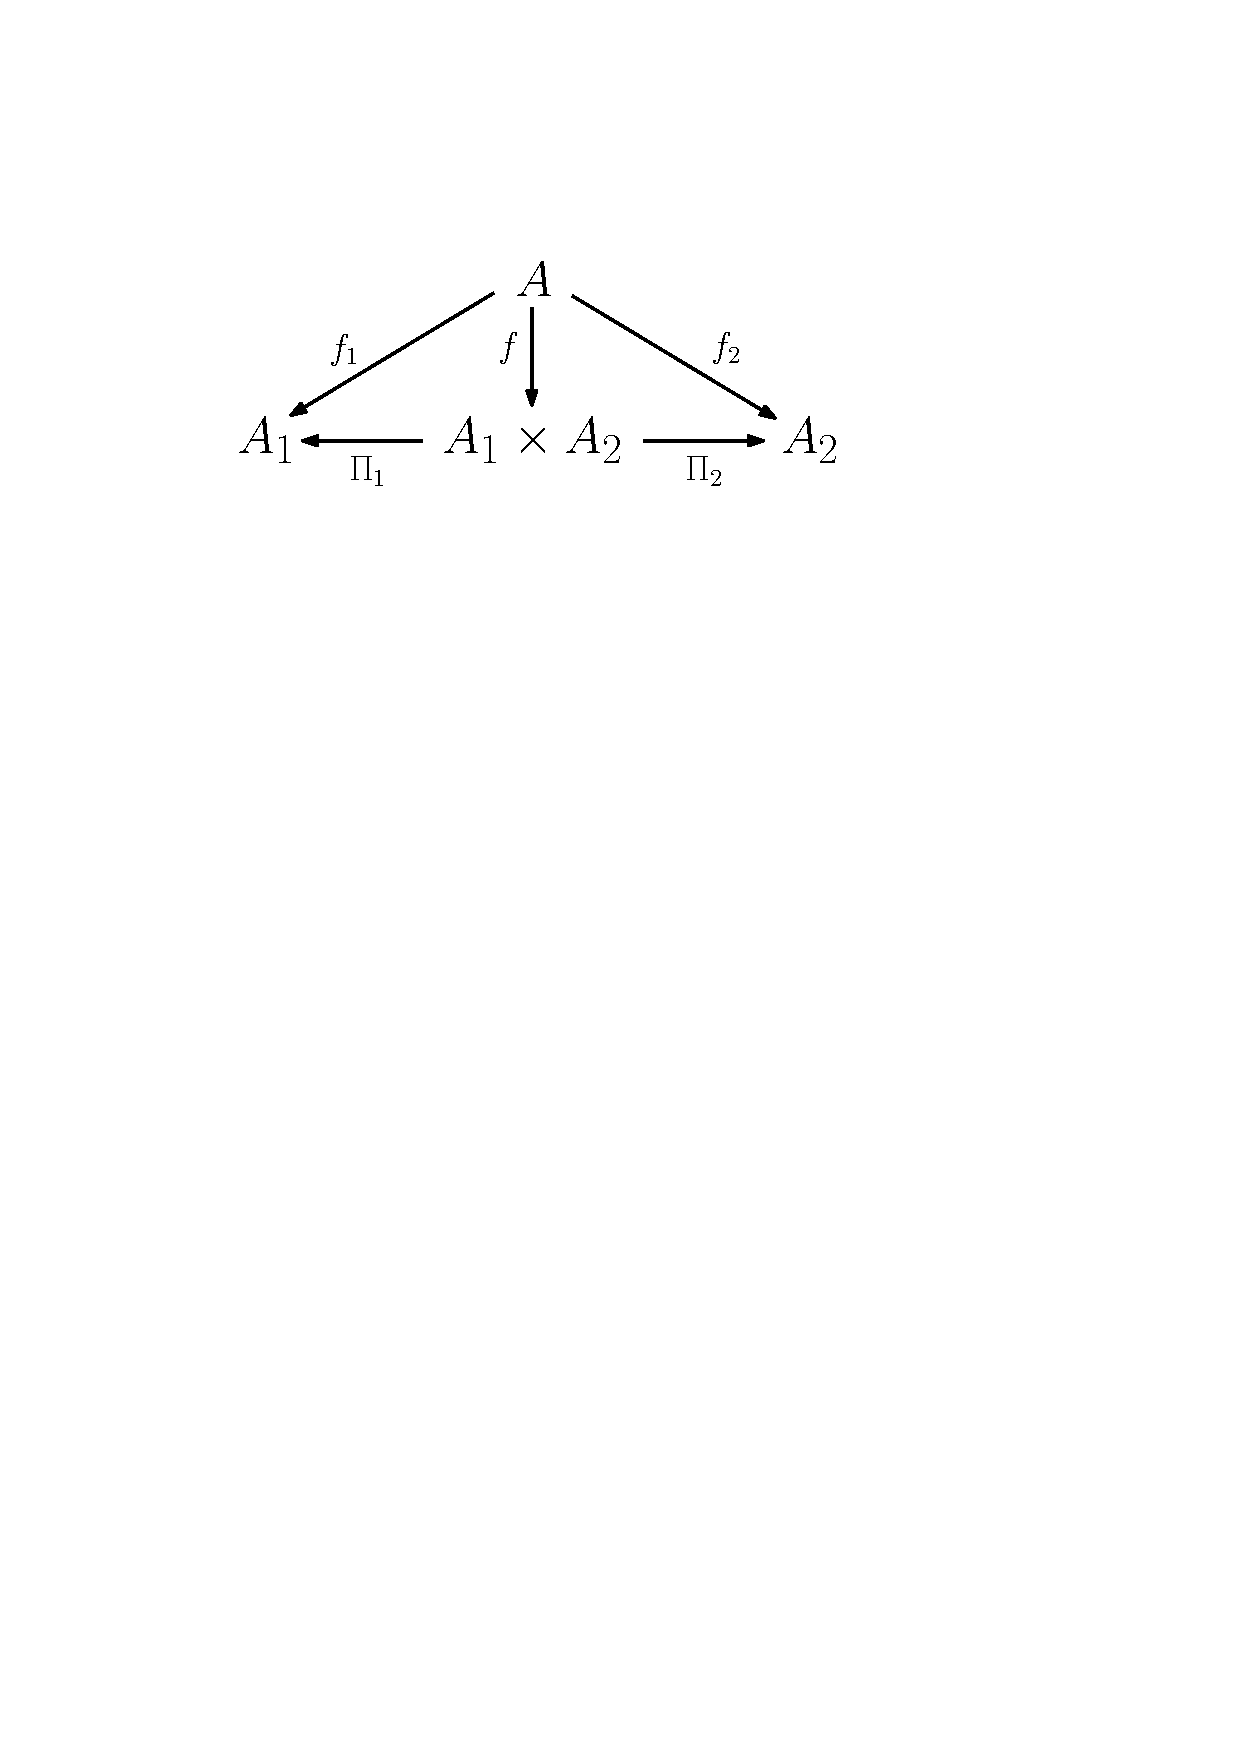
\includegraphics[scale=0.56]{Figures/l5f4_coord.pdf}
\end{figure*}

\begin{exmp}
The function $f:\mathbb{R}^2\rightarrow \mathbb{R}^3$ defined by $f(x,y)=(xy,\,sin(x^2),\,x+y^3)$ has 3 coordinate functions $f_1,f_2,f_3:\mathbb{R}^2\rightarrow \mathbb{R}$ given by 
\begin{alignat*}{3}
&f_1((x,y))=xy, && f_2((x,y))=sin(x^2), \text{ and } && f_3((x,y))=x+y^3.
\end{alignat*}
\end{exmp}

\subsection{Properties of Composition of Functions}
We wish to see whether properties such commutativity and associativity hold for this function operation. It turns out that associativity holds, but commutativity does not always hold for function composition (see Example~\ref{ex_comp}(iv)).
\begin{lem}
Let $A,\,B,\,C,\,D$ be sets and $f:\rightarrow B,\, g:B\rightarrow C$ and $h:C\rightarrow D$ be functions. Then the following are true.
\begin{enumerate}[i)]
\item (Associative law) $(h\circ g)\circ f=h\circ (g\circ f)$.
\item (Identity law) $f\circ 1_A=f$ and $1_B\circ f=f$.
\end{enumerate}
\end{lem}

\section{Inverse Function}
We are interested in finding out conditions for existence of inverse of a function $f$. We will also see that this inverse is unique when it exists.
\begin{defn}[Existence]
Let $A$ and $B$ be sets and let $f:A \to  B$ and $g:B \to A$ be functions. Then the function $g$ is 
\begin{enumerate}[i)]
\item a \textbf{right inverse} for $f$ if $f\circ g=1_B$,
\item a \textbf{left inverse} for $f$ if $g\circ f=1_A$, and
\item an \textbf{inverse} for $f$ if it is both a right and left inverse.
\end{enumerate}
\end{defn}
\begin{rem}If $g$ is a left (right) inverse for $f$, then $f$ is a right (left) inverse for $g$.
\end{rem}

\begin{exmp}
Let $P$ be the set of all people and $W$ be the set of women with at least one child, and let $c:P \to W$ be the function that maps a person to their mother and $m:W \to P$ be the function that maps a woman to her eldest child. 

Choose a person $p\in P$ who is not the eldest of their siblings, and let the eldest sibling of the chosen person be $p'$. Then, $c(p)=w$, for some $w\in W$ and $m(w)=p'\neq p$. Thus, $(m\circ c)(p)\neq p, \forall p\in P$.

Choose a woman $w\in W$. Then, $m(w)=p$ for some $p\in P$ and $c(p)=w$. Thus, $(c\circ m)(w)=w$.

Hence, $m$ has a left inverse ($c$) but no right inverse and $c$ has a right inverse ($m$) but no left inverse.

Had $P$ been the set of people who are eldest of their siblings, then the maps $c$ and $m$ would have been inverse of each other.

Had $m$ been a map from $P$ to $P$, then neither right nor left inverse of either maps would not have existed.
\end{exmp}

\begin{lem}[Uniqueness]
Let $A$ and $B$ be sets, and let $f:A \to B$ be a function.
\begin{enumerate}[i)]
\item If $f$ has an inverse, then it is unique.
\item If $f$ has a right inverse $g$ and a left inverse $h$, then $g=h$, and hence $f$ has an inverse.
\item If $f$ has an inverse $g$, then $g$ has an inverse, which is $f$.
\end{enumerate}
\end{lem}
\begin{proof} Same proof can be used in parts i) and ii). Part iii) is left as an exercise to the reader.
%\begin{enumerate}[i)]
%\item 
Suppose $g,h : B \to A$ are both inverses of $f$. We will show $g=h$. By virtue of being inverses, $g$ and $h$ should be right and left inverse of $f$ respectively. That is, $f \circ g = 1_B$ and $h \circ f = 1_A$. Using associativity of combination of functions, we conclude, 
\begin{align*}
g = 1_A \circ g = h \circ f \circ g = h \circ 1_B = h.
\end{align*}
%\item Use proof of previous part.
%\item Proof is left as an exercise to the reader.
%\end{enumerate}
\end{proof}
\begin{defn}
Let $A$ and $B$ be sets, and let $f:A \to B$ be a function. If $f$ has an inverse, then the inverse is denoted by $f^{-1}: B \to A$.
\end{defn}

\begin{rem} 
\begin{enumerate}
\item $f^{-1}\circ f=1_A$ and $(f^{-1}\circ f)(a)=a,\,\forall a\in A$.
\item $f\circ f^{-1}=1_B$ and $(f\circ f^{-1})(b)=b,\,\forall b\in B$.
\item Given the graph of a function $f:A \to B$, where $A,B\subseteq \mathbb{R}$, the inverse function $f^{-1}$ can be plotted by reflecting the graph of $f$ in the line $x=y$. This is same as first reflecting $f$ in \textit{y-axis} followed by $90^{\circ}$ clockwise rotation.
\end{enumerate}
\end{rem}

\end{document}
